\documentclass[12pt,a4paper]{scrartcl}

%\usepackage{algorithmic}    % Typesetting for pseudocode
%\usepackage{algorithm}      % Formatting for general algorithm blocks
\usepackage{fancyhdr}       % Gives fancy header
\usepackage{mdwlist}        % List related commands
\usepackage{url}            % Nicer URL formatting
\usepackage{new3151defs}    % COMP[39]151 defs
\usepackage{fancyvrb}

% Automata package
\usepackage{tikz}
\usetikzlibrary{arrows, automata, positioning, shapes}

% Page header
%\pagestyle{fancy}
%\lhead{COMP[39]151 Warmup Assignment
%\rhead{Timothy Wiley, z3109831}

% Line spacing 1.6 for 'double'
%\linespread{2}

% Declare commonly used graphic extensions and precedence
\DeclareGraphicsExtensions{.pdf,.png,.jpg}

\begin{document}

\title{COMP[39]151 Assignment 2}
\author{Aditya Keswani (z3242379) \\ 
        \texttt{akeswani@cse.unsw.edu.au} \\ 
        and \\ 
        Timothy Wiley (z3109831) \\
        \texttt{timothyw@cse.unsw.edu.au} }

\maketitle

\section{Definitions and Assumptions}
In order to implement the \emph{Life Stories Exchange} system, we make use of the following definitions and assumptions:
\begin{itemize}
    \item The total number of seniors, denoted as $nSeniors$, is known by all seniors.
    \item Each senior is assigned a unique id, denoted as $id$, in the range $[1,nSeniors]$
    \item Each senior knows the id's of all other seniors they are connected to.
          The predicate $conn(x,y)$ is true if senior $x$ is connected to senior $y$ and false otherwise.
    \item For each ordered pair of connected seniors $(x,y)$ there exists a one-directional message passing channel, $Chan(x,y)$, where senior $x$ sends to senior $y$.
          Therefore, two message passing channels exist between each pair of connected seniors.
\end{itemize}

\section{Description of Algorithm}
Our algorithm uses a round-based system.
Each round iterates through two phases:
\begin{enumerate}
    \item A phase of sending, and
    \item A phase of receiving.
\end{enumerate}

In the sending phase, each senior sends one message, $sendMsg$, to every connected senior with a lower id.
That is:
\begin{equation}
    \forall i, 0 \le i < id, conn(i, id) \quad C(id,i)!sendMsg
\label{eq:send-phase}
\end{equation}

In the receiving phase, each senior receives one message, $recvMsg$, from every senior they are connected to.
Also, each must senior responds, with $respMsg$, to a message received that was sent in the sending phase.
That is:
\begin{align}
    \forall i, 0 \le i \le nSeniors, conn(i, id) &\quad C(i,id)?recvMsg \\
    \forall i, 0 \le i, id < i \le nSeniors, conn(i, id) &\quad C(id,i)!respMsg
\label{eq:recv-phase}
\end{align}

The rounds continue until all seniors are sharing life stories, dead or having a seniors moment.
This sending/receiving process ensures that:
\begin{itemize}
    \item Only one message is send between pairs of connected seniors in the sending phase
    \item Seniors must receive a message from every connected senior.
\end{itemize}
We exploit these properties for our negotiation protocol and for detecting death.

The explanation of the remainder of our algorithm is broken into three components, the negotiation protocol, the senior state machine, and death detection.

\subsection{Negotiation Protocol}
Our protocol to determine which seniors share their life stories is based on the TCP-handshake protocol.
This protocol operates on a pair of seniors $x$ and $y$, with three phases:
\begin{enumerate}
    \item Senior $x$ sends a \emph{request} to senior $y$, which indicates they wish to share their life story.
    \item Senior $y$ responds with an \emph{acknowledgement}, indicating they accept the proposal.
    \item Senior $x$ establishes the sharing by responding with a \emph{confirmation}.
\end{enumerate}

If the three messages are sent, then the two seniors are considered to be sharing life stories.
However, at stages 2 and 3, the seniors may also send a \emph{decline}, indicating they are no longer interested in sharing stories.
Seniors also send a broadcast \emph{finish} message to indicate they are talking to someone else already.

In summary, five types of messages can be sent:
\begin{itemize}
    \item \texttt{MSG\_REQ} - Request to talk
    \item \texttt{MSG\_ACK} - Acknowledge a request to talk
    \item \texttt{MSG\_CONF} - Confirm talking
    \item \texttt{MSG\_DECL} - Decline any request or acknowledgement
    \item \texttt{MSG\_FIN} - The senior is finished and will process no further messages.
\end{itemize}

\subsection{Senior State Machine}
We use a state machine to model the how the stages of the message protocol impact the behaviour senior, shown in Fig. \ref{fig:senior-state-machine}.
The red states and transitions represent the sending phase of the message protocol, while the blue states and transitions represent the receiving phase.

\begin{figure}[h]
   \centering
   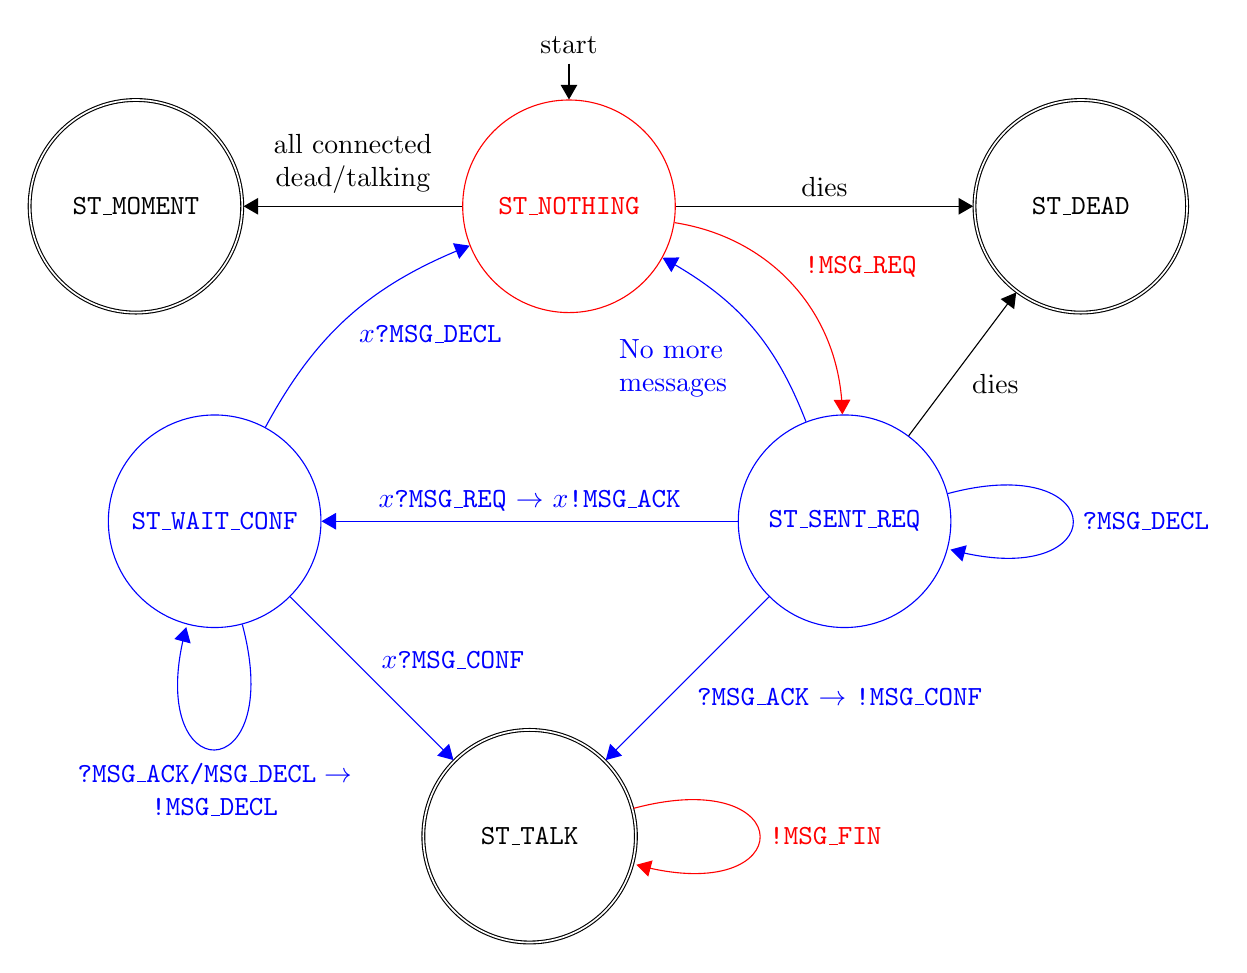
\begin{tikzpicture}[->,>=triangle 60, on grid,auto]

   % Nodes
      \node[state,initial above,minimum size=2.7cm,color=red]    (noth)  at (4.5,8)   {\texttt{ST\_NOTHING}};
      \node[state,accepting,minimum size=2.7cm]        (talk)  at (4,0)     {\texttt{ST\_TALK}};
      \node[state,accepting,minimum size=2.7cm]        (dead)  at (11,8)    {\texttt{ST\_DEAD}};
      \node[state,accepting,minimum size=2.7cm]        (momt)  at (-1.0,8)  {\texttt{ST\_MOMENT}};
      \node[state,minimum size=2.7cm,color=blue]                  (sreq)  at (8,4)   {\texttt{ST\_SENT\_REQ}};
      \node[state,minimum size=2.7cm,color=blue]                  (wcnf)  at (0.0,4)     {\texttt{ST\_WAIT\_CONF}};

   % Paths
      \path (noth) edge [bend left=00]  node[above]       {$\begin{array}{c} \textrm{all connected} \\ \textrm{dead/talking} \end{array}$} (momt)
                   edge [bend left=00]  node[above]       {dies} (dead)
                   edge [bend left=40,color=red]  node[above right] {\texttt{!MSG\_REQ}} (sreq);
      \path (sreq) edge [bend left=00]  node[below right] {dies} (dead)
                   edge [loop right,color=blue]    node[right]       {\texttt{?MSG\_DECL}} (sreq)
                   edge [bend left=00,color=blue]  node[above]       {$x$\texttt{?MSG\_REQ} $\rightarrow$ $x$\texttt{!MSG\_ACK}} (wcnf)
                   edge [bend right=20,color=blue] node[below left]  {$\begin{array}{l} \textrm{No more} \\ \textrm{messages} \end{array}$} (noth)
                   edge [bend left=00,color=blue]  node[below right] {\texttt{?MSG\_ACK} $\rightarrow$ \texttt{!MSG\_CONF}} (talk);
      \path (wcnf) edge [bend left=00,color=blue]  node[above right] {$x$\texttt{?MSG\_CONF}} (talk)
                   edge [loop below,color=blue]    node[below]       {$\begin{array}{c}\texttt{?MSG\_ACK/MSG\_DECL} \rightarrow \\ \texttt{!MSG\_DECL} \end{array}$} (wcnf)
                   edge [bend left=20,color=blue]  node[below right] {$x$\texttt{?MSG\_DECL}} (noth);
      \path (talk) edge [loop right,color=red]    node[right]       {\texttt{!MSG\_FIN}} (talk);
   \end{tikzpicture}
   \caption{Senior State Machine}
   \label{fig:senior-state-machine}
\end{figure}

The state \texttt{ST\_NOTHING} in the default state to which the senior returns if there are no messages to respond to.
This is also the starting point for the sending phase. Once all messages have been sent, the senior enters \texttt{ST\_SENT\_REQ} to perform the receiving phase.
In this state, the following properties are observed:
\begin{itemize}
    \item Messages are received concurrently from all connected seniors.
    \item Received messages are processed sequentially.
    \item The first message that matches one of the valid transitions, causes the senior to change state, but the receiving process continues until completion.
          That is, until a message has been received from every connected senior.
          This is why the state \texttt{ST\_WAIT\_CONF} may receive requests or acknowledgements and needs to send declines in response to them.
\end{itemize}

If the senior transitions into \texttt{ST\_WAIT\_CONF}, then it records the id of the senior which caused the transition, recorded in the variable $x$.
Only receiving a decline or confirmation from senior $x$ will cause a transition out of the waiting state.
Whereas messages from other seniors are rejected.

It should be noted that the sending of the broadcast \texttt{MSG\_FIN} constitutes part of the sending phase.
This is because such messages will not be received until the next receiving phase after they have been sent.
Also, the receiving of these messages is not recorded on the diagram, but it is assumed they do not cause any state transition.

The points at which seniors can die are also strictly maintained.
Seniors cannot die when in the state \texttt{ST\_WAIT\_CONF} as they may not send another message once in this state.
Also, our implementation must ensure that if a senior is to die it does so before entering the state \texttt{ST\_WAIT\_CONF}.

Finally, it should be noted that the state machine ensures that any senior sends an extra \texttt{MSG\_CONF} or \texttt{MSG\_DECL} whenever a connected senior responds their request with an acknowledgement.

\subsection{Death Detection}
To detect death we exploit two properties of our solution:
\begin{itemize}
    \item For each valid channel $Chann(x,y)$ at least one message is sent along it each round.
    \item Reading of messages is performed concurrently
\end{itemize}

Therefore, we place a timeout on reading from a channel.
If this timeout occurs before a message is received, then we can immediately infer the senior we are attempting to receive from has died.

It should be noted that we need to make the timeout large enough to ensure every senior has the opportunity to send their messages.
Also, while messages are received concurrently, they are processed sequentially.
This means we must allow time for the sequential processing to ensure seniors have adequate time to respond.

\section{Verification}
\label{sec:verification}

\subsection{Degree of Death}

\section{Complexity Analysis}
The following facts are used in the complexity analysis:
\begin{itemize}
    \item As noted in section \ref{sec:verification}, at worst, one senior will enter an end state on each round.
    \item Therefore, given $n$ seniors, there will be at most $n$ rounds.
    \item Also in each round, each senior receives $k-1$ messages, where $k$ is the number of remaining seniors.
\end{itemize}

\subsection{Message Complexity}
In each round, at worst, $(k-1)^2 = O(k^2)$ messages a sent amongst the remaining seniors.
Given at most $n$ round, the message complexity is $\sum_{i=1}^n (i-1)^2$, which is $O(n^3)$

\subsection{Time Complexity}
As the workload is a constant factor of the number of messages received, $O(k)$ work is done by each senior, making $O(k^2)$ work done per round.
Therefore, given at most $n$ rounds, the total Time Complexity is $O(n^3)$

\end{document}
